
The Standard Model of particle physics (SM) is a Quantum Field Theory (QFT) describing the known fundamental particles and their interactions. It accounts for three of the four known fundamental force - electromagnetism, the weak nuclear force, and the strong nuclear force, but not gravity. Further, the SM describes a mechanism for combining the weak and electromagnetic forces into a singular interaction, known as the electroweak force. It is a non-Abelian gauge theory, invariant under the Lie Group $SU(3)_C\bigotimes SU(2)_L\bigotimes U(1)_Y$, where $C$ refers to color charge, $L$, the helicity of the particle, and $Y$, the hypercharge.

%%%%%%%%%%%%%%%%%%%%%%%%%%%%%%%%%%%%%%%%%%%%%%%%%%%%%%%%%%%%%%%
\subsection{The Forces and Particles of the Standard Model}
\label{sec:forcesParticles}

The SM particles, summarized in Figure \ref{fig:SM_summary}, can be classified into two general categories based on their spin: fermions, and bosons. 

\begin{figure}[H]
\centering
   \includegraphics[width=0.75\linewidth]{figures/theory/SM_summary.pdf}
\caption{A summary of the particles of the Standard Model, including their mass, charge and spin, with the fermions listed on the left, and the bosons on the right. \cite{oerter2006the}}
\label{fig:SM_summary}
\end{figure}

Fermions are particles with $\frac{1}{2}$-integer spin, which according to the spin-statistics theorem, causes them to comply with the Pauli-exclusion principle. They can be separated into two groups, leptons and quarks, each of which consist of three generations of particles with increasing mass.

Leptons are fermions interact via the electroweak force, but not the strong force. The three generation of leptons consist of the electron and electron neutrino, the muon and muon neutrino, the tau and tau neutrino. The quarks, which do interact via the strong force - which is to say they have color charge - in addition to the electroweak force. The three generations include the up and down quarks, the strange and charm quarks, and the top and bottom quarks. Each of these generations form left-handed doublets invariant under $SU(2)$ transformations. For the leptons these doublets are:

\begin{equation}
  \label{eq:lepDoublets}
  \begin{pmatrix}
    e^{-} \\
    \nu_e \\
  \end{pmatrix}_L,\:  
  \begin{pmatrix}                                                                                                                                   \mu^{-} \\
    \nu_\mu \\     
  \end{pmatrix}_L,\: 
  \begin{pmatrix}                                                                                                                             
    \tau^{-} \\
    \nu_\tau \\                                                    
  \end{pmatrix}_L
\end{equation}

And for the quarks:

\begin{equation}        
  \label{eq:quarkDoublets}
  \begin{pmatrix}                                                                                                                               
    u \\                                                                                                                                  
    d \\                                                                                                                                  
  \end{pmatrix}_L,\:                                                                                                                           
  \begin{pmatrix}                                                                                         
    s \\                                         
    c \\                                                                                                                             
  \end{pmatrix}_L,\:                                                                                                                           
  \begin{pmatrix}     
    t \\                                                                                                                            
    b \\                                                                                                                            
  \end{pmatrix}_L                
\end{equation}

For both leptons and quarks, the heavier generations can decay into the lighter generation of particles, while the first generation does not decay. Hence, ordinary matter generally consists of this first generation of fermions - electrons, up quarks, and down quarks. Each of these fermions has a corresponding anti-particle, which has an equal mass as its partner but oppsite charge. The fermions acquire their mass via the Higgs Mechanism, except for the neutrinos, whose mass has been experimentally confirmed but is not accounted for in the SM. 

Bosons, by contrast, have integer spin, and are therefore unconstrained by the Pauli-exclusion principle. The SM includes two kinds of bosons: Gauge bosons, which are spin-1 particles that mediate the interactions between the fermions, and a single scalar, i.e. spin-0, particle - the Higgs Boson. Of the gauge bosons, the $W^+$, $W^-$ and $Z$ bosons - which are the mass eigenstates of the electroweak bosons - mediate the weak interaction, while the photon mediates the electric force, and the gluon mediates the strong force. 

%%%%%%%%%%%%%%%%%%%%%%%%%%%%%%%%%%%%%%%%%%%%%%%%%%%%%%%%%%%%%%%

\subsection{The Higgs Mechanism}
\label{sec:higgsMech}

A key feature of the SM is the gauge invariance of its Lagrangian. However, any terms added to the Lagrangian giving mass to the the gauge bosons would violate the underlying symmetry of the theory. This presents a clear problem with the theory: The experimental observation that the W and Z bosons have mass seems to contradict the basic structure of the SM. 

Rather than abandoning gauge invariance, an alternative way for particles to acquire mass beyond adding a simple mass term to the Lagrangian was theorized by Higgs, Englert and Brout in 1964 \cite{Higgs}. This procedure for introducing masses for the gauge bosons while preserving local gauge invariance, known as the Higgs mechanism, was incorporated into the electroweak theory by Weinberg in 1967 \cite{PhysRev.127.965}.  

\subsubsection{The Higgs Field}
\label{sec:higgsField}

The Higgs mechanism introduces a complex scalar $SU(2)$ doublet, $\Phi$, with the form:

\begin{equation}
  \label{eq:phiDoublet}
  \Phi = 
  \begin{pmatrix}                                                                                                           
    \phi^+ \\                                                                                                               
    \phi^0 \\                                                                                                                            
  \end{pmatrix}_L                                                                                                                    
\end{equation}

This field introduces a scalar potential to the Lagrangian of the form:

\begin{equation}
  \label{eq:higgsV}
  V(\Phi) = \mu^2|\Phi^\dagger\Phi| + \lambda (|\Phi^\dagger \Phi|)^2
\end{equation}

Where $\mu$ and $\lambda$ are free parameters of the new field. This represents the most general potential allowed while preversing $SU(2)_L$ invariance and renormalizability. In the case that $\mu^2 < 0$, this potential takes the form shown in Figure \ref{fig:higgspotential}.

\begin{figure}[H]
\centering
   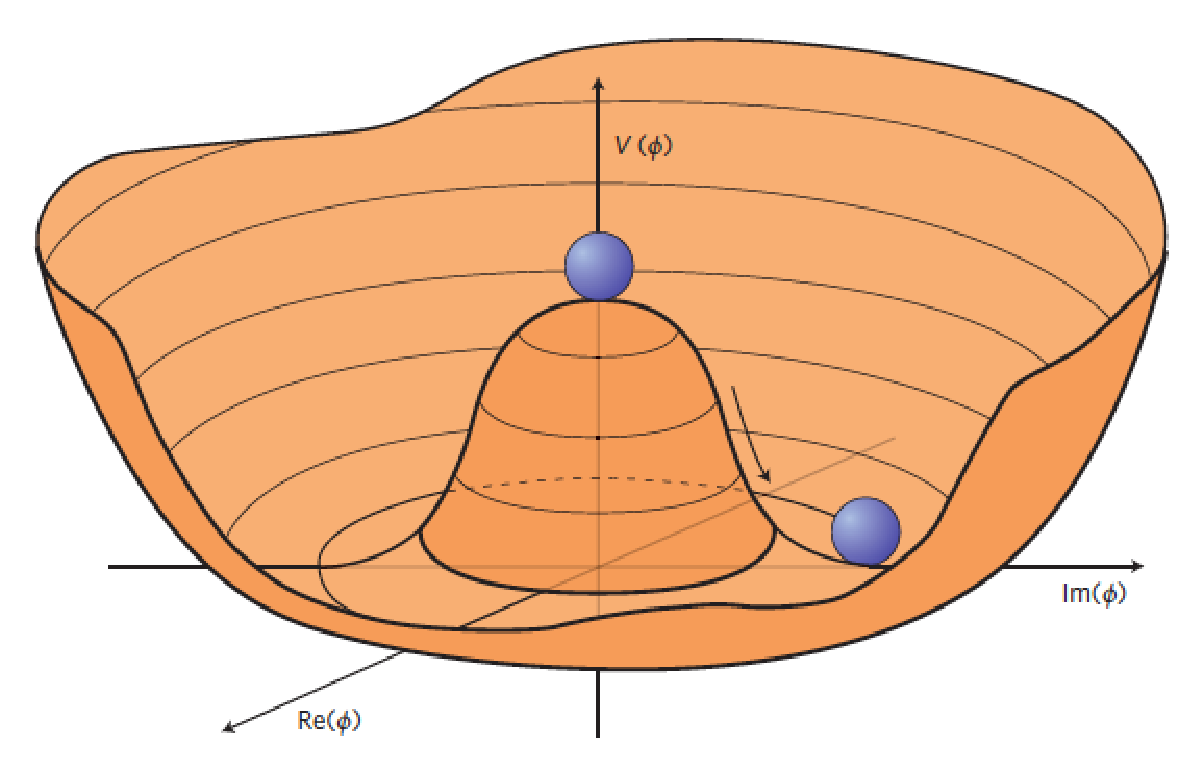
\includegraphics[width=0.75\linewidth]{figures/theory/higgspotential.eps}
\caption{The value of the Higgs potential, $V(\Phi)$ as a function of $\Phi$, for the case that $\mu^2 < 0$ \cite{Ellis:1638469}.}
\label{fig:higgspotential}
\end{figure}

The significant feature of this potential is that its minimum does not occur for a value of $\Phi = 0$. Instead, it is minimized when $|\Phi^\dagger \Phi| = -\mu^2/\lambda$. This means that in its ground state, the Higgs field takes on a non-zero value - referred to as a vacuum expectation value (VEV). So while the Higgs potential is globally symmetric, about the minimum this symmetry is broken. Since the minimum is determined only by $\Phi^\dagger \Phi$, there is some ambiguity in the particular definition of the VEV, but it is generally represented as 

\begin{equation}
  \label{eq:VEV}
  \left\langle\Phi\right\rangle = \frac{1}{\sqrt{2}}
  \begin{pmatrix}                                                                                                                               
    0 \\                                                                                                                                   
    v \\                                                                                                                                   
  \end{pmatrix}                                                                                                                       
\end{equation}

The full value of $\Phi$ can be written as 

\begin{equation}                                                                                                                                
  \label{eq:HandV}                                                                                                                                  \left\langle\Phi\right\rangle = \frac{1}{\sqrt{2}}                                                                     
  \begin{pmatrix}                                                                                                                               
    0 \\                                                                                                                   
    v + H/\sqrt{2}\\                                               
  \end{pmatrix}                                                                                                                        
\end{equation}

with $v$ being the value of the VEV, and $H$ being the real value of the scalar field. 

%%%%%%%%%%%%%%%%%%%%%%%%%%%%%%%%%%%%%%%%%%%%%%%%%%%%%%%%%%%%%%%
\subsubsection{Electroweak Symmetry Breaking}
\label{sec:EWKbreaking}

The Electroweak (EWK) interaction is described in the SM by a $SU(2)_L\bigotimes U(1)_Y$ gauge theory. This theory predicts three $SU(2)_L$ gauge boson, $W^1_\mu$, $W^2_\mu$, $W^3_\mu$, and a single $U(1)_Y$ gauge boson, $B_\mu$. The couplings of these bosons to the Higgs field show up in the kinetic terms of the scalar field $\Phi$ in the Lagrangian:

\begin{equation}
  \label{eq:Lphi}
  (D_\mu\Phi)^\dagger(D^\mu\Phi) = |(\partial_\mu - \frac{ig}{2}W^a_\mu\sigma^a - \frac{ig'}{2}B_\mu Y)\phi|^2
\end{equation}

Here $D_\mu$ represents the covariant derivative required to preserve gauge invariance, $g$ and $g'$ represent coupling constant of the gauge bosons, $\sigma^a$ denotes the Pauli matrices of $SU(2)$, and $Y$ represents the hypercharge of $U(1)$. The terms in this interaction which contribute to the masses of the gauge bosons can be written as:

\begin{equation}
  \label{eq:LVEV}
  \frac{1}{2}(0,v)(\frac{g}{2}W^a_\mu\sigma^a - \frac{g'}{2}B_\mu)^2
  \begin{pmatrix}                                                                                                                               
    0 \\                                                                                                                                        
    v \\                                                                                                                                        
  \end{pmatrix}
\end{equation}

Expanding these terms into the mass eigenstates of the electroweak interaction yields four physical gauge bosons, two charged and two neutral, which are linear combinations of the fields $W^1_\mu$, $W^2_\mu$, $W^3_\mu$, and $B_\mu$:

\begin{equation}
\begin{gathered}
  \label{eq:EWKfields}
  W^\pm_\mu = \frac{1}{\sqrt{2}}(W^1_\mu \pm i W^2_\mu) \\
  Z^\mu = \frac{1}{\sqrt(g^2+g'^2)}(-g'B_\mu + gW^3_\mu) \\
  A^\mu = \frac{1}{\sqrt(g^2+g'^2)}(gB_\mu + g'W^3_\mu) \\
\end{gathered}
\end{equation}

And the masses of these fields are given by:

\begin{equation}
\begin{gathered}
  \label{eq:EWKmasses}
  M^2_W = \frac{1}{4}g^2v^2 \\
  M^2_Z = \frac{1}{4}(g^2+g'^2)v^2 \\
  M^2_A = 0 \\
\end{gathered}
\end{equation}

This produces exactly the particles we observe - three massive gauge bosons and a single massless photon. The massless photon represents the portion of the gauge symmetry, a single $U(1)$ of the electromagnetic force, that remains unbroken by the VEV.

Interactions with the Higgs field also lead to the generation of the fermion masses, which in the Lagrangian take the form:

\begin{equation}
  \label{eq:Lfermion}
  -\lambda_\psi (\bar{\psi}_L \phi \psi_R + \bar{\psi}_R \phi^\dagger \psi_L)
\end{equation}

After symmetry breaking has occured and $\phi$ has taken on the value of the VEV as written in equation \ref{eq:VEV}, the mass terms or the fermions become $\lambda_\psi v$. Written this way, the fermion masses are proportional to their Yukawa coupling to the VEV, $\lambda_\psi$. 

Based on the equation \ref{eq:HandV}, an additional mass term, $\mu^2H^2$ arises from the potential $V(\Phi)$. This term can be understood as anexcitation of the Higgs field, a scalar boson with mass $M_H = \mu$. This is the Higgs boson, which comes about as a natural prediction of electroweak symmetry breaking. 

The fermion's Yakawa coupling to the VEV take the same form as the fermion's coupling to the Higgs boson - $\lambda_\psi$. Therefore, the strength of a fermion's interaction with the Higgs is directly proportional to its mass. We now have a model that predicts a Higgs boson with mass $M_H = \mu$, which interacts with the fermions with coupling strength $\lambda_\psi$. Because $\mu$ and $\lambda_\psi$ are free parameters of the theory, the mass of the Higgs boson and its interactions with the fermions must be measured experimentally. 

%%%%%%%%%%%%%%%%%%%%%%%%%%%%%%%%%%%%%%%%%%%%%%%%%%%%%%%%%%%%%%%

\subsection{$t\bar{t}H$ Production}
\label{sec:ttH_theory}

The strength of a particles interaction with the Higgs, given by its Yakawa coupling, is proportionate to its mass. The top quark - as the heaviest known particle - has the strongest interaction, making this interaction particularly interesting to study. While several processes involve interactions between the Higgs and the top, some Higgs production modes include the top interaction only as a part of a loop diagram, such as the gluon-gluon fusion diagram shown in Figure \ref{fig:Hgg}. This process therefore only allows for an indirect probe of the Higgs-top Yakawa coupling, as the flavor of the quark in this diagram is not unique.

\begin{figure}[H]
\centering                                                                                                                
   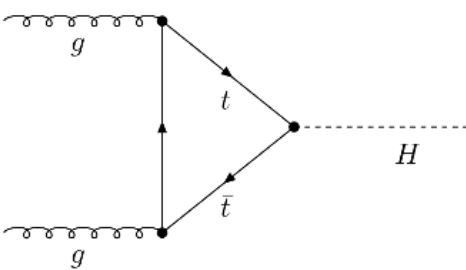
\includegraphics[width=0.6\linewidth]{figures/theory/Hgg.JPG}
\caption{Diagram of a Higgs boson produced via gluon-gluon fusion.}
\label{fig:Hgg}
\end{figure}

Studying the Higgs produced in association with top quark pairs, $t\bar{t}H$, allows this interaction to be measured directly. This process, as shown in Figure \ref{fig:ttH_diagram}, involves a unique coupling between the Higgs and the top, which can be identified by the top quark pair in the final state.

\begin{figure}[H]
\centering
   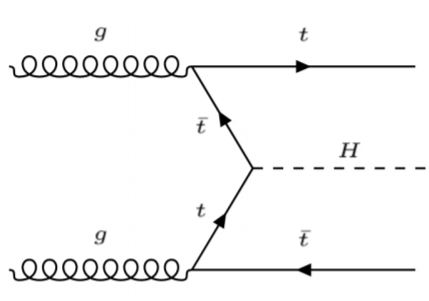
\includegraphics[width=0.6\linewidth]{figures/theory/ttH_diagram.JPG}
\caption{Diagram of a Higgs boson produced in association with a pair of top quarks.}                         
\label{fig:ttH_diagram}                                                                                    
\end{figure}

The Higgs boson, as well as the top quarks, have very short lifetimes - on the order of $10^{-22}$ s and $10^{-25}$ s respectively - meaning they can only be observed via their decay products. This thesis focuses on $t\bar{t}H$ events with multiple leptons in the final state, $t\bar{t}H-ML$. This includes $H \rightarrow W^+W^-$ events, where at least one of the W bosons decays leptonically. 

While the branching ratio of $H\rightarrow W^+W^-$ is smaller than $H \rightarrow b \bar{b}$, it produces a clearer signal. On the other hand, $H\rightarrow \gamma\gamma$ produces the most easily identifiable signal, but has a much smaller branching ratio than $H\rightarrow W^+W^-$. Therefore, compared with other final state, the $t\bar{t}H-ML$ channel is an attractive candidate for study, as it involves a good balance between statistical power and identifiability. 

%%%%%%%%%%%%%%%%%%%%%%%%%%%%%%%%%%%%%%%%%%%%%%%%%%%%%%%%%%%%%%%

\subsection{WZ + Heavy Flavor Production}
\label{sec:WZ_theory}

Part \ref{part:wz} is dedicated to a measurement of WZ produced in association with a heavy flavor jet - namely, a charm or b-jet - in the fully leptonic channel. In the instance that both the W and Z bosons decay leptonically, this process produces a final state similar to $t\bar{t}H$, making it an irreducible background for $t\bar{t}H-ML$ specifically, and any analysis that includes multiple leptons and b-tagged jets in the final state. 

\begin{figure}[H]
  \includegraphics[width=0.35\linewidth]{figures/wz_3l.png}%
  \includegraphics[width=0.35\linewidth]{figures/wz_3l_c.png}%
  \includegraphics[width=0.29\linewidth]{figures/wz_bbar.JPG}
  \caption{Example Feynman diagrams of WZ + heavy flavor production}
  \label{fig:wz_feynman}
\end{figure}

The b-jets produced in this process can be thought of in two different way: either as originating from the quark ``sea'' of the initial state hadrons, or as the result of gluons from the colliding protons splitting into $b\bar{b}$ pairs. However, the heavy flavor contribution to the parton distribution function (PDF) of the proton is uncertain, and simulations of this process disagree depending on which of these two approaches one considers. This makes WZ + heavy flavor difficult to accurately simulate, and introduces a large uncertainty for any analysis which includes it as a background, motivating a measurement of this process.

%%%%%%%%%%%%%%%%%%%%%%%%%%%%%%%%%%%%%%%%%%%%%%%%%%%%%%%%%%%%%%%  

\subsection{Extensions to the Standard Model}
\label{sec:bsm}

While the SM has been tested to great precision, particularly at the LHC, it is generally accepted that it is only valid up to a certain energy scale. It is assumed that above a certain energy, at the scale where something like a Grand Unified Theory (GUT) or quantum gravity become relevant, the SM will not be applicable. Further, there are several experimental observations that the SM fails to explain. For example, the SM predicts neutrinos to be massless, despite experimental observation to the contrary, and fails to explain the observation of dark matter and dark energy. 

Another example, revelant to the Higgs sector, is known as the hierarchy problem: large quantum corrections to the Higgs mass from loop diagrams, such as those shown in Figure \ref{fig:hierarchyDiagram}, are many orders of magnitude larger than the Higgs mass itself. The observed value of the Higgs mass therefore requires extremely precise cancellation between these corrections and the bare mass of the Higgs, a cancellation which seems unnatural and suggests something missing in our theoretical picture.

\begin{figure}[H]
\centering
   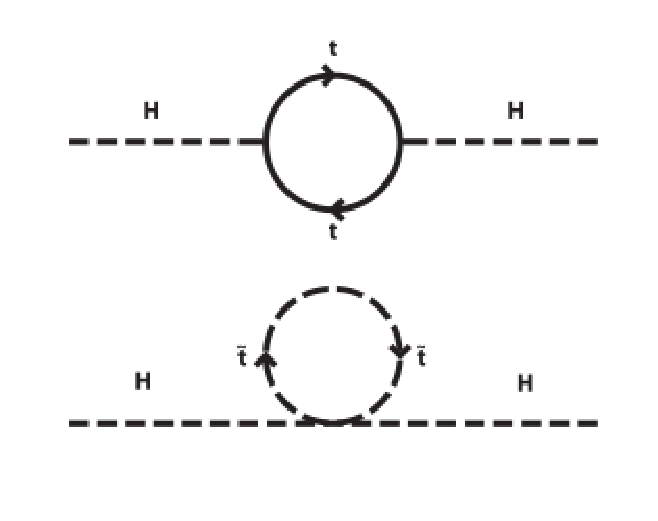
\includegraphics[width=0.5\linewidth]{figures/theory/hierarchyDiagram.eps}
\caption{Above diagram is the leading order correction to the Higgs mass via a top quark loop, and below is the stop squark loop, coming from a supersymmetric extension of the SM, that provides a potential cancellation of the top diagram.}
\label{fig:hierarchyDiagram}
\end{figure}

Because so many of the properties of the Higgs boson have not yet been studied, its interactions are a promising place to search for new physics that could resolve some of the limitations of the SM. As explained above, the interactions of the Higgs with the top quark, as in $t\bar{t}H$ production, are particularly interesting: As the most massive particle in the Standard Model, the top quark is the most strongly interacting with the Higgs. Therefore, any new physics effects are likely to be seen most prominently in this interaction.

These interactions can be measured directly by studying the production of a Higgs Boson in association with a pair of Top Quarks ($t\bar{t}H$). While this process has been observed by both the ATLAS \cite{ttH_paper} and CMS \cite{Sirunyan_2018} collaborations, these analyses have focused on measuring the overall rate of $t\bar{t}H$ production. There are several theories of physics Beyond the Standard Model (BSM), however, that would affect the kinematics of $t\bar{t}H$ production without altering its overall rate \cite{Dumont_2013}.

An Effective Field Theory approach can be used to model the low energy effects of new, high energy physics, by paramaterizing BSM effects as higher dimensional operators. These additional operators can then be added to the SM Lagrangian to write an effective Lagrangian that accounts for the effects of these higher energy physics. The lowest order of these that could contribute to Higgs-top coupings are dimension-six, as represented in Equation \ref{eq:dim6}.

\begin{equation}
\label{eq:dim6}
\mathcal{L}_{eff} = \mathcal{L}_{SM} + \frac{f}{\Lambda}\mathcal{O}^6
\end{equation}

Here $\Lambda$ represents the energy scale of the new physics, and $f$ is a Wilson coefficient which represents the strength of the effective coupling. An experimental observation of any non-zero value of $f$ would be a sign of BSM physics.

The addition of these operators can be shown to modify the transverse momentum ($p_T$) spectrum of the Higgs Boson in Higg-top interactions, without effecting the overall rate of $t\bar{t}H$ production \cite{Banerjee_2014}. The effect of these higher order effects on the  as shown in Figure \ref{fig:eft_pt}. 

\begin{figure}[H]
\centering
   \includegraphics[width=0.5\linewidth]{figures/theory/higgs_pt.PNG}
\caption{The momentum spectrum of the Higgs boson produced via top-quarks with (red) and without (blue) the presence of dimension-six operators.}
\label{fig:eft_pt}
\end{figure}


This provides a clear, physics observable that could be used to search for BSM effect. Therefore, reconstructing the momentum spectrum of the Higgs in $t\bar{t}H$ events provides a means to observe new physics in the Higgs sector.


%%%%%%%%%%%%%%%%%%%%%%%%%%%%%%%%%%%%%%%%%%%%%%%%%%%%%%%%%%%%%%% 

